% This is samplepaper.tex, a sample chapter demonstrating the
% LLNCS macro package for Springer Computer Science proceedings;
% Version 2.21 of 2022/01/12
%
\documentclass[runningheads]{llncs}
%
\usepackage[T1]{fontenc}
% T1 fonts will be used to generate the final print and online PDFs,
% so please use T1 fonts in your manuscript whenever possible.
% Other font encondings may result in incorrect characters.
%
\usepackage{graphicx}
% Used for displaying a sample figure. If possible, figure files should
% be included in EPS format.
%
% If you use the hyperref package, please uncomment the following two lines
% to display URLs in blue roman font according to Springer's eBook style:
\usepackage{color}
\usepackage{hyperref}
\renewcommand\UrlFont{\color{blue}\rmfamily}
\urlstyle{rm}
%

\usepackage{amssymb}
\newcommand{\tx}{\mathsf{tx}}
\newcommand{\TX}{\mathsf{TX}}
\newcommand{\comment}[1]{\textcolor{red}{\textbf{Comment by Zhuo:} #1}}
\newcommand{\thtime}{\Delta_{\mathsf{th}}}
% message time is \Delta
\newcommand{\synctime}{\Delta_{\mathsf{sync}}}
\renewcommand{\ts}{\mathsf{ts}}
\newcommand{\nset}{\mathcal{I}}
\usepackage{xcolor}
\newcommand{\allset}{\mathcal{S}}
\newcommand{\hset}{\mathcal{H}}
\newcommand{\aset}{\mathcal{A}}
\begin{document}
%
\title{Transaction Order Fairness in Synchronous Networks}
%
%\titlerunning{Abbreviated paper title}
% If the paper title is too long for the running head, you can set
% an abbreviated paper title here
%
% \author{Zhuo Cai\inst{1}\orcidID{0000-0001-9673-6888} \and
% Amir Kafshdar Goharshady\inst{2}\orcidID{0000-0003-1702-6584}}
% %
% \authorrunning{Z. Cai and A. Goharshady}
% First names are abbreviated in the running head.
% If there are more than two authors, 'et al.' is used.
%
% \institute{Hong Kong University of Science and Technology, HKSAR, China \email{zcaiam@connect.ust.hk} \and
% University of Oxford, Oxford, UK 
% \email{goharshady@cs.ox.ac.uk}}
%
\maketitle              % typeset the header of the contribution
%
\begin{abstract}
The abstract should briefly summarize the contents of the paper in
150--250 words.

\keywords{First keyword  \and Second keyword \and Another keyword.}
\end{abstract}
%
%

\section{Introduction}
Blockchain systems have gained significant attention in recent years. The central problem of blockchain is to extend an ordered chain of transactions and reaching consensus among decentralized nodes. While many consensus protocols have been proposed to solve this problem, most of them only consider consistency and liveness properties. Consistency means every node have the same view of the chain or its prefix. Liveness means that new transactions are eventually added to the chain. 

One important yet little studied property is \emph{fairness} in transaction ordering. Fairness means that the order of transactions in the chain should reflect the order in which they were received by the nodes. This property is important for several reasons. First, it helps prevent attacks by manipulating the order of transactions, such as front-running attacks and sandwich attacks. Second, it ensures that users have a fair chance of having their transactions included in the chain. The challenge to achieve transaction order fairness lies in the fact that nodes may receive transaction requests at different times due to network delays. It is nontrivial to reach consensus on the order of transactions being received, especially in the presence of malicious nodes that may try to manipulate the order for their own benefit. 

The formal study of transaction order fairness was initiated by the seminar work of Kelkar et al. \cite{DBLP:conf/crypto/Kelkar0GJ20}. They defined \textit{receive-order-fairness} which requires all honoest nodes to output a transaction $\tx$ before another transaction $\tx'$ if sufficiently many nodes receive $\tx$ before $\tx'$. This fairness definition intuitively corresponds to the notion of ``first received, first output''. Kelkar et al. showed that the definition is impossible to achieve due to a scenario called Condorcet paradox which causes a non-transitive global ordering even when all local orderings are transitive. In the example of $n$ nodes and $n$ transactions, node $1$ receives transactions in the order $[\tx_1, \tx_2,\dots, \tx_n]$ and each other node $i$ in the order of $[\tx_i, \tx_{i+1}, \dots, \tx_n, \tx_1, \dots, \tx_{i-1}]$. We have that $n-1$ nodes receive $\tx_j$ before $\tx_{j+1}$ for $j$ in $1,\dots, n$. However, $n-1$ nodes receive $\tx_n$ before $\tx_1$. This creates a cycle in the global ordering: $\tx_1 \prec \tx_2 \prec \dots \prec \tx_n \prec \tx_1$. 

To circumvent this impossibility, Kelkar et al. proposed a relaxed definition called \textit{block-order-fairness}. It states that when sufficiently many nodes receive $\tx$ before $\tx'$, then no honest node can deliver $\tx$ in a block after $\tx'$. The relaxation allows $\tx$ to be placed after $\tx'$ as long as they are delivered in the same block. This relation evade the Condorcet paradox by placing paradoxical orderings into the same block. It gives malicious miners sufficient flexibility to manipulate the order of transactions. For example, if the attacker finds a transaction $\tx_1$ that is suitable for a front-running attack by a transaction $\tx_2$, the attack will be successful when the miner adds both transactions into the same block with $\tx_2$ before $\tx_1$. Such a block is valid as long as it includes all transactions received between $\tx_1$ and $\tx_2$. This implies that the attacker has suffcient time to prepare its attack transaction $\tx_2$, up to the time to generate a block. In blockchain systems where consensus/finality on blocks is achieved within each slot, the block time at least includes a few rounds of messages propagating among the network.  They presented a protocol called $\mathsf{Aequitas}$ that achieves the block-order-fairness. 

\comment{In Ethereum PoS, the delay to generate a block is $1\Delta$, because block proposers must receive the old block before producing the new block. It is not $2\Delta$ (to also receive enough votes on the old block) because Ethereum PBFT style consensus only runs once in an epoch. \newline However, Ethereum plans to achieve SSF (single-slot-finality). Each block time consists of the time to conduct two phases of voting. So a block time will be much longer than message delay time. \newline In consensus that supports transaction ordering, voting-consensus per slot is necessary. } 

One limitation of block-order fairness is that it allows malicious miners to re-order transactions within each block even if there is no paradoxical ordering. In other words, it is designed to withstand the worst case paradoxical ordering, such as a paradoxical cycle that takes up an entire block, but cannot achieve best-effort fairness when it is not the worst case. Kiayias et al. \cite{DBLP:conf/eurocrypt/KiayiasLS24} presents a more fine-grained relaxation of receive-order-fairness, which they call \textit{bounded unfairness}. Bounded unfairness parameterized by a bound $B$ states that for two transactions $\tx,\tx'$, if sufficiently many nodes receive $\tx$ before $\tx'$, then $\tx$ cannot be placed more than $B$ transactions later compared to $\tx'$. Bounded unfairness tries to find the minimum $B$. When $B$ is much smaller than the number of transactions in a block, it allows for a more fine-grained control over transaction ordering compared to block-order-fairness. Moreover, they showed the connection between finding the minimum bound $B$ and finding the directed bandwidth of a graph. As a result, the problem is NP-hard and also hard to approximate for an constant ratio. 

Kiayias et al. \cite{DBLP:conf/eurocrypt/KiayiasLS24} also presents a variation of their protocol to handle long paradoxical cycles. Assuming transaction dissemination delay is bounded by $\Delta_{\tx}$, they showed that $B$ is bounded by at most $3$ times the maximum number of transactions disseminated concurrrently within a $\Delta_{\tx}$ time window. They use median timestamp to order these transactions and achieve \textit{timed-directed-bandwidth-fairness}. 

Regarding performance, their protocol, called $\mathsf{Taxis}$, runs exponentially on the number of edges of the subgraph of the transaction graph that is defined by the (largest) Condorcet cycle. This is undesirable in practice. 


In this work, we present another fairness notion, which we call \textit{time-delayed-fairness}. We relax from receive-order-fairness differently, by changing to condition to impose a pairwise ordering requirement. Our fairness parameterized by delay $\thtime$ states that if sufficiently nodes receive $\tx$ at least $\thtime$ time before $\tx'$, then $\tx$ should be delivered before $\tx'$. We also analyze the parameter $\varphi$, the threshold for ratio of nodes for a transaction to be considered ``receive'' before another. Assuming a transaction dissemination delay of $\synctime$, we show that our fairness gets rid of the Condorcet paradox under suitable parameter choices. In detail, it is $\thtime>\synctime/k$ when $\varphi>1-h/k$, where $h$ is the ratio of honest nodes and $k$ is a positive integer. Compared with $\mathsf{Aequitas}$, our protocol is more fine-grained and achieves the best-possible fairness when there are few Condorcet cycles. Compared with $\mathsf{Taxis}$, our protocol runs in polynomial time and achieves concretely better time delayed fairness. 

\comment{It's good to have an example. Given a sequence, we output better ordering. }


\begin{definition}[Time-Delayed-Fairness]\label{def:timed-fairness}
    A protocol achieves time-delayed-fairness with parameters $\thtime$ and $\varphi$ if for any two transactions $\tx$ and $\tx'$, if at least $\varphi$ fraction of honest nodes receive $\tx$ at least $\thtime$ time before receiving $\tx'$, then every honest node delivers $\tx$ before $\tx'$.
\end{definition}


\section{Related Works} \label{sec:related}
\section{Possibility Result} \label{sec:result}

In this section, we present our main possibility result for achieving time-delayed-fairness assuming the network is synchronous and ignore communication and computation cost. 


\paragraph{Notations} Throughout the paper, when we assume the network is synchronous, we use $\synctime$ to denote the maximum dalay for a transaction to be disseminated to all honest nodes after it is sent by a honest node. We use $\thtime$ to denote the time-delay parameter in our time-delayed-fairness definition. We use $n$ to denote the total number of nodes and $h$ to denote the ratio of honest nodes. Use $\allset$, $\hset$ and $\aset$ to denote the set of all nodes, the set of honest nodes, and the set of adversary nodes. We use $\varphi$ to denote the threshold ratio for a transaction $\tx$ to be considered as received before another transaction $\tx'$. 

\paragraph{Synchrony assumption} In this section, we assume the network is synchronous with parameter $\synctime$.  

\paragraph{Adversary model} We assume a static Byzantine adversary that can corrupt up to $n(1-h)$ nodes, where $h>2/3$. The adversary can coordinate the corrupted nodes to deviate from the protocol in any way. The adversary can also delay or reorder messages sent by honest nodes, but cannot forge messages. 

\paragraph{Notation - Timestamp} For a node $i$, denote its timestamp for a transaction $\tx$ as $\ts_i(\tx)$. In our setting, guaranteed by Byzantine broadcast, if an honest node confirms a valid timestamp $\ts_i(\tx)$ by node $i$, all other nodes confirm the same timestamp $\ts_i(\tx)$ for node $i$ receiving $\tx$. If node $i$ does not broadcast its timestamp for $\tx$, it is considered missing, all honest nodes infer that node $i$ will receive $\tx$ in the future if $\tx$ is ever disseminated. 

\paragraph{Notation - Precede relation} For two transactions $\tx$ and $\tx'$, the set of $n$ nodes $\allset$ participating in the transaction ordering scheme, denote $\nset_{\thtime}(\tx, \tx')$ as the set of nodes that receive $\tx$ at least $\thtime$ before $\tx'$, i.e., $\nset_{\thtime}(\tx, \tx') = \{i\in \allset: \ts_i(\tx) + \thtime\le \ts_i(\tx')\}$. We say there is a ($\thtime, \varphi$)-precede relation between $\tx$ and $\tx'$, denoted as $\tx \prec_{\thtime, \varphi} \tx'$, if $|\nset_{\thtime}(\tx, \tx')| \ge n\varphi$. When the context is clear, we omit the subscripts and simply write $\nset(\tx, \tx')$ and $\tx \prec \tx'$. Using the above notation, time-delayed-fairness requires that for any pair of two transactions $\tx$ and $\tx'$ such that $\tx\prec \tx'$,  $\tx$ should be delivered before $\tx'$. 

\paragraph{Protocol Design} Transaction ordering protocols in this section do not consider communication and computation cost, in order to achieve time-delayed-fairness with the tightest parameters possible. For every node, upon receiving a transaction, it records the time of receiving the transaction and runs a Byzantine broadcast protocol for the transaction along with its timestamp. Under the assumption that the network is $\synctime$-synchronous and more than $2/3$ nodes are honest, Byzantine broadcast protocols terminate in bounded time when the broadcaster is honest.  By Byzantine broadcast, if an honest node $i$ confirms a transaction $\tx$ with timestamp $t$ from a node $j$, all other honest nodes also confirm that node $j$ receive $\tx$ at time $t$. Therefore, all honest nodes have the same view of the time when each node receives a transaction. Our trsanction ordering mechanism outputs an order of transactions based on the view of timestamps of all nodes and existing part of blockchain, which are the same in the view of all honest nodes. Therefore all honest nodes output the same new block and consensus of blockchain is achieved. Such protocol is highly inefficient in practice. In later sections, we will discuss more efficient protocols to order transactions that meet our time-delayed-fairness. 

\paragraph{Feasibility and Precede Loop} Time-delayed-fairness with paramter $\thtime$ nad $\varphi$ is possible if and only if there is no sequence of transactions $\tx_1, \tx_2, \ldots, \tx_k$ such that $\tx_1\prec \tx_2$, $\tx_2\prec \tx_3$, $\ldots$, $\tx_{k-1}\prec \tx_k$ and $\tx_k\prec \tx_1$. We call such sequence a ($\thtime, \varphi$)-precede loop. If there is a ($\thtime, \varphi$)-precede loop, then time-delayed-fairness with parameters $\thtime$ and $\varphi$ is impossible because the ordering of transactions in the loop contradicts with each other. If there is no ($\thtime, \varphi$)-precede loop, then time-delayed-fairness with parameters $\thtime$ and $\varphi$ can be achieved by topologically sorting the directed graph formed by all transactions as nodes and all ($\thtime, \varphi$)-precede relations as directed edges. 

\paragraph{Paramter space for $\varphi$} For the time-delayed-fairness to be meaningful, $\varphi$ should be in the range $(1-h, h]$. If $\varphi\leq 1-h$, then the adversary has enough votes to impose an arbitrary order of any two transactions even though all honest nodes receive them in opposite order. If $\varphi>h$, then even if all honest nodes receive transaction $\tx$ at least $\thtime$ before transaction $\tx'$, they do not have enough vote to impose a constraint to deliver $\tx$ before $\tx'$ when the adversary do not cooperate. 

\paragraph{Monotonicity of feasible parameters} If time-delayed-fairness can be achieved with parameters $\thtime$ and $\varphi$, then it can also be achieved with parameters $\thtime'\geq \thtime$ and $\varphi'\geq \varphi$. This is because if $\tx\prec_{\thtime', \varphi'} \tx'$, then $\tx\prec_{\thtime, \varphi} \tx'$. Therefore, an ordering of transactions that satisfies time-delayed-fairness with parameters $\thtime$ and $\varphi$ also satisfies time-delayed-fairness with parameters $\thtime'$ and $\varphi'$. 

\begin{theorem}{(Feasible thresholds)}\label{thm:threshold}
    Under $\synctime$-synchronous network, in a system  where $h$ fraction of nodes are honest, for any positive integer $k$ such that $1-h/k\le h$, i.e., $k\le h/(1-h)$, time-delayed-fairness cannot be achieved with parameters $\thtime\le\synctime/k$ and $\varphi \le 1-h/k$, and can be achieved with parameters $\thtime>\synctime/k$ and $\varphi>1-h/k$.
\end{theorem}

We first prove the theorem \ref{thm:threshold} for the special case when $k=1$. The infeasible part is trivial because when $\varphi\le 1-h$, time-delayed-fairness is impossible because the adversary can impose an arbitrary order of any two transactions. The feasible part is proved as analyzing the time window for all honest nodes to receive each transaction. Our $\synctime$-synchrony assures that for each transaction, the timestamps of all honest nodes receiving it fall into a time window of size $\synctime$. Assume for the sake of contradiction that there is a ($\thtime, \varphi$)-precede loop $\tx_1\prec \tx_2$, $\tx_2\prec \tx_3$, $\ldots$, $\tx_{l-1}\prec \tx_l$ and $\tx_l\prec \tx_1$. For each transaction $\tx_i$, let $[s_i, e_i]$ be the time window for all honest nodes to receive $\tx_i$. For simplicity, define a transaction $\tx_{l+1}$ as the same as $\tx_1$. For each $i$ in $1,2,\dots, l$, since $\tx_i\prec\tx_{i+1}$, at least $\varphi(>1-h)$ nodes receive $\tx_i$ at least  $\thtime(>\synctime)$ before $\tx_{i+1}$, and at least one node $n_i$ is honest. By definition of the time windows, $\ts_{n_i}(\tx_i)\ge s_i$ and $\ts_{n_i}(\tx_{i+1})\le e_{i+1}$. By precede relation we have $\ts_{n_i}(\tx_i)\le \ts_{n_i}(\tx_{i+1})-\thtime < \ts_{n_i}(\tx_{i+1})-\synctime$. Chaining the inequalities, we have $s_i\le \ts_{n_i}(\tx_i)<\ts_{n_i}(\tx_{i+1})-\synctime \le e_{i+1} - \synctime$. In short, $s_i<e_{i+1}-\synctime$. Since $e_i-s_i\le \synctime$ and $e_{i+1}-s_{i+1}\le \synctime$, we have $s_i<s_{i+1}$ and $e_i<e_{i+1}$. This implies $s_1<s_{l+1}=s_1$, which is a contradiction. 


Now we prove the theorem \ref{thm:threshold} for the case when $k$ is an integer larger than $1$. (1) For the infeasible result of $\thtime\le \synctime/k$ and $\varphi\le 1-h/k$, we can show the existence of a precede loop consisting of $k$ transactions. Suppose there is an ordering of the $n$ nodes. For each transaction $\tx_i$ ($1\le i\le k$), the first $1-(i/k)h$ fraction of nodes receive $\tx_i$ at time $(i/k)\synctime$, and the remaining $(i/k) h$ fraction of nodes receive $\tx_i$ at time $(i/k-1)\synctime$.  This construction does not violate the $\synctime$-synchrony assumption, as for each $\tx_i$ the timestamps fall into a $\synctime$-sized time window. Now we show that $\tx_i\prec \tx_{i+1}$, among the first $1-(i/k)h$ fraction of nodes that receive $\tx_i$ at time $(i/k)\synctime$, $1-((i+1)/k)h$ fraction of nodes receive $\tx_{i+1}$ at time $((i+1)/k)\synctime$, which is at least $\thtime$ after $(i/k)\synctime$. For the last $(i/k)h$ fraction of nodes that receive $\tx_i$ at time $(i/k)\synctime-\synctime$, they all receive $\tx_{i+1}$ at time $((i+1)/k)\synctime-\synctime$. Therefore, the fraction of nodes in $\nset(\tx_{i},\tx_{i+1})$ is $(1-((i+1)/k)h + (i/k)h)=1-h/k\ge \varphi$. The precede relation $\tx_i\prec \tx_{i+1}$ holds for all $1\le i\le k$. These $k$ transactions form a precede loop. 

(2) For the feasible result of $\thtime > \synctime/k$ and $1-h/k<\varphi\le h$, we use a more fine-grained time-window analysis. Assume for the sake of contradiction that there is a ($\thtime, \varphi$)-precede loop $\tx_1\prec \tx_2\cdots \prec \tx_l \prec \tx_1$. For each precede relation $\tx_i\prec \tx_{i+1}$, more than $1-h/k$ fraction of nodes are in $\nset(\tx_{i}, \tx_{i+1})$. This implies that less than $h/k$ fraction of nodes are not in $\nset(\tx_{i}, \tx_{i+1})$. In particular, less than $hn/k$ honest nodes are not in $\nset(\tx_{i}, \tx_{i+1})$, which account for less than $1/k$ fraction of all honest nodes. Assuming the earliest timestamp of all honest nodes receiving $\tx_1$ is $0$, then by precede relation $\tx_1\prec\tx_2$, more than $(k-1)/k$ fraction of honest nodes receive $\tx_2$ at or after $\thtime>\synctime/k$. The remaining less than $1/k$ fraction of honest nodes receive $\tx_2$ after $(1/k-1)\synctime$ due to $\synctime$-synchrony. This induction is generalized in the following lemma \ref{lem:induction}. 

\begin{lemma}\label{lem:induction}
    Under $\synctime$-synchronous network, in a system  where $h$ fraction of nodes are honest, under time-delayed-fairness parameters $\thtime>\synctime/k$ and $\varphi > 1-h/k$, for any integer $i\in \{0,1,\dots, k-1\}$, if $\tx_{1}\prec \tx_{2}$ and at least $(k-i)/k$ fraction of honest nodes receive $\tx_1$ at or after some time $t$, which also implies that the other at most $i/k$ fraction of honest nodes receive $\tx_1$ at or after $t-\synctime$, then more than $(k-i-1)/k$ fraction of honest nodes receive $\tx_{2}$ after $t_{2}=t+\thtime>t+\synctime/k$. The remaining less than $(i+1)/k$ fraction of honest nodes receive $\tx_{2}$ after $t+(1/k-1)\synctime$.
\end{lemma}

\begin{proof}
    Among the at least $(k-i)/k$ fraction of honest nodes that receive $\tx_1$ at or after time $t$,  more than $(k-i)/k-1/k=(k-i-1)/k$ fraction of honest nodes are in $\nset(\tx_1, \tx_2)$, hence receiving $\tx_2$ at or after $t+\thtime$. The remaining less than $(i+1)/k$ fraction of honest nodes receive $\tx_2$ at or after $t+(1/k-1)\synctime$ due to $\synctime$-synchrony. 
\end{proof}

We can apply lemma \ref{lem:induction}. For example, given that more than $(k-1)/k$ fraction of honest nodes receive $\tx_2$ after time $t+\synctime/k$, we can infer that more than $(k-2)/k$ fraction of honest nodes receive $\tx_3$ after time $t+2\synctime/k$.  By repeatedly applying the lemma we show that for any integer $i\in \{2,\dots, k+1\}$, more than $i+1$  We argue that the first $j$ is at least $k+1$, because by induction at least $(k-i+1)/k$ fraction of honest nodes receive $\tx_i$ after $t+(i-1)\synctime/k$ for $i\le j$.  Therefore, we conclude that at least all honest nodes receive $\tx_{j}$ after time $t+((j-1)/k-1)\synctime\ge t$. 

{
\color{brown}

\begin{theorem}{(Feasible parameters)} \label{thm:possibility}
    Under $\synctime$-synchronous network, in a system  where $h$ fraction of nodes are honest, time-delayed-fairness can be achieved with parameters $\thtime$ and $\varphi$ if $\thtime>\synctime/k$ and $\varphi>1-h/k$ for some positive integer $k$. As as special case when $k=1$, time-delayed-fairness can be achieved when $\thtime>\synctime$ and $\varphi>1-h$.

    This result is tight in the sense that time-delayed-fairness with parameters $\thtime$ and $\varphi$ cannot be achieved if for any integer $k\ge 1$, either $\thtime\leq \synctime/k$ or $\varphi\leq 1-h/k$.
\end{theorem}

The set of feasible parameters are better illustrated at figure \ref{fig:params}. The green shaded area is the feasible region. The boundary lines are $\thtime=1/k$ and $\varphi=1-h/k$ for positive integers $k$. The dashed line is $\varphi=1-h/\lceil 1/\thtime \rceil$. For any point above the dashed line, it is feasible. For any point on or below the dashed line, it is infeasible.

\begin{figure}[htp]
    \centering
    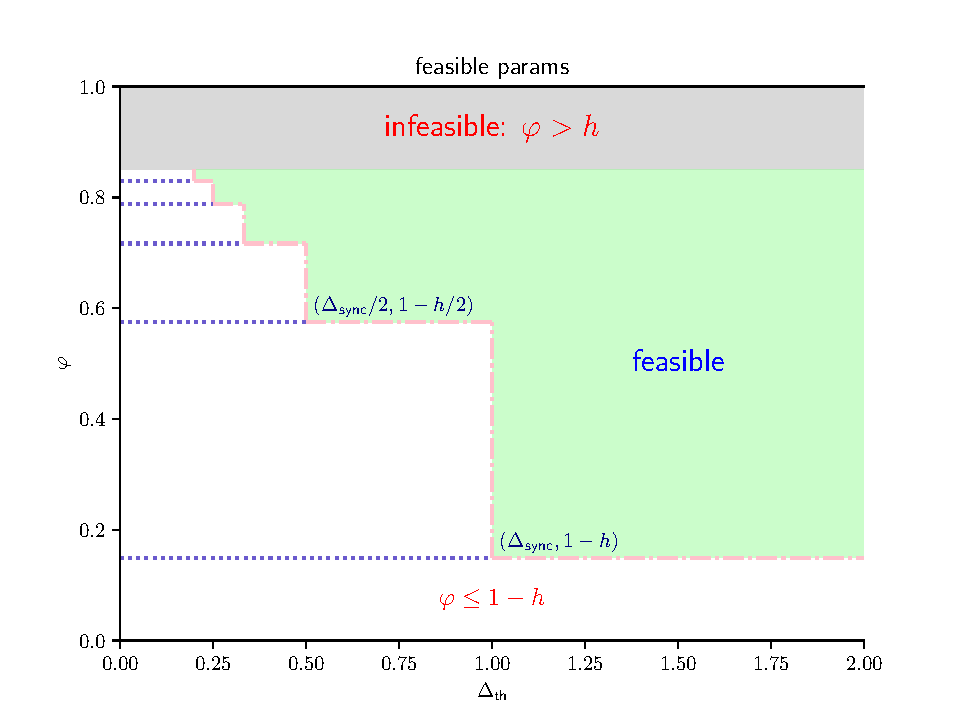
\includegraphics[width=0.7\textwidth]{plots/param.pdf}
    \caption{The set of feasible parameters $(\thtime, \varphi)$ for time-delayed-fairness, where $\synctime=1$ and $h=0.7$. The green shaded area is the feasible region. The boundary lines are $\thtime=1/k$ and $\varphi=1-h/k$ for positive integers $k$. The dashed line is $\varphi=1-h/\lceil 1/\thtime \rceil$. For any point above the dashed line, it is feasible. For any point on or below the dashed line, it is infeasible. }
    \label{fig:params}
\end{figure}

\begin{proof}
    In order to prove the theorem, we need to show that (1) for any paramters in green shaded area of figure \ref{fig:params}, i.e., for any positive integer $k$, when $\thtime>\synctime/k$ and $\varphi>1-h/k$, time-delayed-fairness can be achieved; (2) for any parameters in white area of figure \ref{fig:params}, i.e., (2a) for any positive integer $k$, when $\thtime\leq \synctime/k$ or $\varphi\leq 1-h/k$, time-delayed-fairness cannot be achieved.
\end{proof}

Maybe it works for any rational number $k=\frac{k_1}{k_2}\ge1$. $k_1,k_2$ are coprime positive integers. 


Do we need to exclude bad reports?  No for the case of $k=1$. 


\subsection{Feasibility for $(\thtime>\synctime, \varphi>1-h)$ and Infeasibility for $(\thtime\leq \synctime, \varphi\leq 1-h)$}

}



\section{END HERE ==== BELOW IS INVALID}
\subsection{System Model}
\paragraph{Nodes/Committee} Assume a committee of $n$ nodes is responsible for processing transactions in the blockchain system. 

\paragraph{Communication} Unless otherwise stated, we assume the communication network is synchronous, i.e., there is a known upper bound $\Delta$ on the time it takes for a message to be delivered from one node to all other nodes. In other words, for each transaction request, every committee node receives it. Moreover, the first node to receive the transaction receives the request at most $\Delta$ time before the last node receives it. 

\paragraph{Adversary Model} Unless otherwise stated, we assume that a small set of nodes is controlled by an arbitrary adversary. Let $h$ be the ratio of honest nodes, and $m=1-h$ be the ratio of malicious nodes. Let $H$ be the set of honest nodes and $M$ be the set of malicious nodes. We require that $h$ is at least larger than $1/2$. In some cases, we require $h$ to be larger than a higher threshold. 

\paragraph{Notations} Let $N = \{1, 2, \dots, n\}$ denote the set of committee nodes. Let $\tx$ denote a transaction and $\TX$ denote the universe of transactions. Let $t_i:\TX\to \mathbb{R}$ denote the mapping from a transaction $\tx$ to the time at which node $i\in N$ receives the transaction. We assume that $t_i(\tx)$ is defined for all nodes $i\in N$.

\paragraph{Timestamp Report} A timestamp report for a node $i$, $R_i$, is a list of tuples $(\tx, t_i(\tx))$ for a subset of transactions that node $i$ has received. Note that malicious nodes might report timestamps different from the actual time they received the transactions. Therefore, we use $t_i(\tx)$ to denote the reported timestamp of transaction $\tx$ by node $i$, and use $\tilde{t}_i(\tx)$ to denote the actual time of node $i$ receiving $\tx$. 

\paragraph{Transaction Ordering Mechanism} A transaction ordering mechanism $\Gamma$ for $n$ nodes, is a function that takes as input a set of timestamp reports from all nodes and outputs a total ordering of the transactions appearing in the timestamp reports. In application, every node should report all transactions that it has received but has not been included in previous blocks yet. Malicious nodes might not share their reports, in which case the ordering mechanism $\Gamma$ use default empty reports for these nodes. 




\subsection{Definition}
We define a new relaxation of the transaction order fairness property, which we call \emph{($\gamma,\delta$)-transaction order fairness}, parameterized by a ratio $\gamma\in (1/2,1)$ and a duration $\delta>0$. We introduce more notations before presenting the definition. 

\paragraph{More Notations} Let $I^{\delta,\{R_i\}_{i\in N}}(\tx_1, \tx_2):=\{i\in N: t_i(\tx_1) \le t_i(\tx_2)-\delta \}$ denote the set of nodes that receive transaction $\tx_1$ at least $\delta$ time before they receive transaction $\tx_2$. If a node does not report to receive $\tx_1$ or $\tx_2$, it is not considered in the set $I^{\delta,\{R_i\}_{i\in N}}(\tx_1, \tx_2)$. When it is clear from the context, we will omit $\delta$ and the set of timestamp reports $\{R_i\}_{i\in N}$ and simply write $I(\tx_1, \tx_2)$.

The definition is as follows: 
\begin{definition}[$(\gamma,\delta)$-Transaction Order Fairness]
A transaction ordering mechanism $\Gamma$ is said to satisfy \emph{($\gamma,\delta$)-transaction order fairness} if the following conditions hold:
\begin{itemize}
\item \emph{Fairness Condition:} For any two different transactions $\tx_1, \tx_2\in \TX$, if $|I(\tx_1, \tx_2)|\ge \gamma n$, which we denote as a constraint relation $\tx_1\prec \tx_2$, then $\Gamma$ outputs $\tx_1$ before $\tx_2$.
\end{itemize}
\end{definition}


\begin{lemma}
A $(\gamma,\delta)$-transaction order fairness mechanism $\Gamma$ exists, if and only if there is no list of transactions $\tx_1, \tx_2,\dots, \tx_k$ such that $\tx_1\prec \tx_2\cdots \prec \tx_k \prec \tx_1$. 
\end{lemma}

Notation: we call a list of transactions $\tx_1, \tx_2,\dots, \tx_k$ such that $\tx_1\prec \tx_2\cdots \prec \tx_k \prec \tx_1$ as a \emph{precede cycle}.

\begin{proof} 
    (1) If there exists a mechanism $\Gamma$, for any list of transactions $\tx_1, \tx_2,\dots, \tx_k$ such that $\tx_1\prec \tx_2\cdots \prec \tx_k \prec \tx_1$, then $\Gamma$ should output $\tx_1$ before $\tx_2$, $\tx_2$ before $\tx_3$, ..., and $\tx_k$ before $\tx_1$. This is a contradiction, since the output of $\Gamma$ is a total ordering of transactions.
    (2) Now assume there is no list of transactions $\tx_1, \tx_2,\dots, \tx_k$ such that $\tx_1\prec \tx_2\cdots \prec \tx_k \prec \tx_1$. We observe that for any set of transactions, one of it is not constraint to be preceded by other transactions, since otherwise every transaction is preceded by some other transaction so that a precede cycle exists. We can construct a mechanism $\Gamma$ by repeating the following: pick one transaction $\tx$ from the set of all unpicked transactions, such that there is no transaction $\tx'$ such that $\tx'\prec \tx$. $\Gamma$ outputs transactions by the order they are picked. 
\end{proof}

\paragraph{Basic bounds for $\gamma$} We naturally require that $\gamma$ be in $(m, h]$. If $\gamma$ is smaller than $m$, then malicious nodes can always report they receive a transaction $\tx_1$ before another transaction $\tx_2$ while honest nodes report the opposite. $\tx_1\prec\tx_2$ and $\tx_2\prec\tx_1$ can both hold, which leads to a precede cycle, so that no mechanism achieves our fairness property. If $\gamma$ is larger than $h$, if malicious nodes always report the opposite of (the majority of) honest nodes, then the number of nodes that report to receive $\tx_1$ before $\tx_2$ is at most $h n$, which is smaller than $\gamma n$. No meaningful precede constraint is placed on the transactions, and the mechanism can output any order of transactions. 

In some cases (small $\delta$ or asynchronous network), we require $\gamma$ to be larger than $1/2$ to avoid the possibility of $\tx_1\prec \tx_2$ and $\tx_2\prec \tx_1$ both holding. In other cases (synchronous network and large $\delta$), self-cycle is impossible even for $\gamma\in (m, 1/2]$. 

\section{Results under the Synchronous Network Model}

In this section, we assume that the synchronous delay is $\Delta$, i.e., whenever an honest node receives a transaction $\tx$ at time $t$, all other honest nodes receive the transaction within the range $[t-\Delta, t+\Delta]$. More precisely, a transaction is received by honest nodes within a $\Delta$-time window $[t', t'+\Delta]$, by picking $t'$ as the earliest time for an honest node to receive it. 

\paragraph{Pruning} Due to the above assumption, a transaction ordering mechanism can prune the reports. If more than $mn$ nodes report to receive a transaction $\tx$ at or before time $t$, then the mechanism can prune the reports of all nodes that report to receive $\tx$ at time larger than $t+\Delta$. This is because if an honest node receives $\tx$ by $t$, other nodes must have received it by $t+\Delta$. Similarly, if more than $hn$ nodes report to receive a transaction $\tx$ at or after time $t$, then the mechanism can prune the reports of all nodes that report to receive $\tx$ at time before $t-\Delta$. If a node is pruned, its report is completely discarded. Pruning only excludes malicious nodes. Pruning is applied exhaustively, until no more pruning can be applied. In subsequent steps of pruning, the pruning threshold is defined as $n'-hn$ where $n'$ is the number of remaining valid reports. This is safe because we only exclude malicious nodes in pruning. 


% \begin{lemma}
% If after pruning, among the remaining valid reports, say $n'$ valid reports, if more than $mh'$ nodes report to receive a transaction $\tx$ at or before time $t$, then any report that reports $\tx$ at time after $t+\Delta$ has been pruned. Similarly, if more than $mn-(n-n') =n'-hn$ nodes report to receive a transaction $\tx$ at or after time $t$, then any report that reports $\tx$ at time before $t-\Delta$ has been pruned.
% \end{lemma}
%
%The proof is obvious by the definition of pruning. 

At the end of exhaustive pruning, we have a set of valid reports. Let $n'$ be the number of valid reports. $n-n'$ nodes are excluded, all of which are malicious nodes. The number of remaining honest nodes is $hn$ and the number of remaining malicious nodes is $n'-hn$. We claim that if more than $n'-hn$ nodes report to receive $\tx$ by time $t$, then all valid reports receive $\tx$ by time $t+\Delta$. Similarly, if more than $n'-hn$ nodes report to receive $\tx$ after time $t$, then all valid reports receive $\tx$ after time $t-\Delta$. The threshold $n'-hn$ translates to a ratio of $1-(n/n')h$. $1-(n/n')h \le 1-h = m$. 


 
\paragraph{Missing transactions and truncation} The set of transactions reported by different nodes might be different. A mechanism needs a rule to handle missing transactions. The main possible issue is missing a preceding constraint. More specifically, $\tx_1$ and $\tx_2$ are reported by some nodes in the current slot, but a precede relation $\tx_1\prec \tx_2$ lacks attestation in the current slot. In the next report slot, some others nodes report $\tx_1$ or $\tx_2$ for the first time and reports to receive $\tx_1$ before $\tx_2$ by $\delta$.  In this section, we assume all nodes share a world clock and send reports at exactly pre-specified time. 

We use the following general solution: transaction ordering mechanisms only consider transactions that have been received by at least $hn$ nodes $\Delta$ time before the prescribed report time.  For example, if a report is scheduled at time $t$, then the mechanism only considers transactions that have been received by at least $hn$ nodes before time $t-\Delta$. We prove that transactions ordered by such a mechanism will not violate precede constraints in future slots. Proof by contradiction, if $\tx_1\prec \tx_2$ but the mechanism (1) outputs $\tx_2$ before $\tx_1$, or (2) outputs $\tx_2$ but not $\tx_1$. In case (1), at least $hn$ nodes received $\tx_1$ by $t-\Delta$, by pruning all reports of nodes that received $\tx_1$ after $t$ are pruned. The same applies to $\tx_2$. This implies that all valid reports of $\tx_1$ and $\tx_2$ are already considered. (2) Since $\tx_2$ is output, at least $hn$ nodes received $\tx_2$ by $t-\Delta$, by pruning, all valid reports received $\tx_2$ by $t$. If $\tx_1\prec \tx_2$, then all valid reports received $\tx_1$ by $t-\delta$, which should appear in the reports of the current slot. 

\paragraph{Constructive Mechanism vs General Mechanism} There are two flavors to show existence of transaction order fairness mechanisms. The first is to construct a mechanism that satisfies the fairness property, which we call a \emph{constructive mechanism}. The second is to show that no precede cycle exists, and then use a general mechanism to order the transactions. 

\subsection{Two simple mechanisms: arbitrary timestamp and median timestamp}
We present two simple mechanisms. The first is to simply select an honest node to broadcast its local timestamps of receiving transactions. How to make sure the proposal is honest? If more than $mn$ nodes object to the proposal, then the proposal is not honest. Nodes object to the proposal if after comparing the proposal with their own timestamps and find any transaction $\tx$ such that the proposal reports to receive $\tx$ at more than $\Delta$ time away from their own timestamps. Such a mechanism can be easily adopted in practice, by asking the validators to attach their local timestamps in their proposals and asking the committee to not vote for proposals that have inconsistent timestamps. This simple mechanism satisfies the fairness property for $\gamma\in(m,h]$ and $\delta\in(4\Delta,+\infty)$. If a precede relation $\tx_1\prec \tx_2$ exists, then an honest node receives $\tx_1$ before $\tx_2$ by $\delta>4\Delta$. According to $\Delta$-synchrony, all honest nodes receive $\tx_1$ before $\tx_2$ by $2\Delta$. If a node tries to put $\tx_2$ before $\tx_1$ in the proposal, then it is considered invalid by all honest nodes. 

The second computes the median timestamp over nodes of every transaction, then orders the transactions by their median timestamps. If two transactions have the same median timestamp, we break the tie by hashes of the transactions. 

The median timestamp mechanism uses pruning and completely discard invalid reports. The median is defined as the median among valid reports. For transactions appearing in some but not all valid reports, we compute the median timestamp by considering missing timestamps as $+\infty$. By truncation, for every transaction that the mechanism outputs, at least $hn>n/2$ timestamps are received so that its median timestamp is one of the actually reported timestamps (not $+\infty$).  

\subsection{Deprecated: $(\gamma\in(m,h], \delta\in[2\Delta,+\infty))$-fairness exists}

For any sequence of transactions $\tx_1, \tx_2, \dots, \tx_k$ such that $\tx_1\prec \tx_2\prec \cdots \prec \tx_k$, we show that $\tx_k \prec \tx_1$ does not hold. 
\begin{proof}
For any $\tx_i$ and $\tx_{i+1}$, $\tx_i\prec \tx_{i+1}$ implies that at least one honest node $j$ satisfies $t_j(\tx_{i}) \le t_j(\tx_{i}) - \delta$. For any other honest node $j'$, we have $t_{j'}(\tx_{i}) \le t_j(\tx_{i}) + \Delta$ and $t_{j'}(\tx_{i+1}) \ge t_j(\tx_{i+1}) - \Delta$. Therefore, we have $t_{j'}(\tx_i) \le t_{j'}(\tx_{i+1}) - (\delta - 2\Delta) \le t_{j'}(\tx_{i+1})$. This implies all honest nodes receive $\tx_{i}$ before $\tx_{i+1}$. Therefore, all honest nodes receive $\tx_{1}$ before $\tx_{k}$. $I(\tx_{k}, \tx_{1})$ is a subset of malicious nodes $M$. Therefore, $|I(\tx_{k}, \tx_{1})|\le mn < \gamma n$. 
\end{proof} 


\subsection{Deprecated: $(\gamma\in(1/2,h], \delta\in(\Delta,+\infty))$-fairness exists}
We show that the median timestamp mechanism satisfies transaction order fairness for $\gamma\in(1/2,h]$ and $\delta\in(\Delta,+\infty)$. We show that whenever $\tx_1\prec \tx_2$, the median timestamp of $\tx_1$ is smaller than that of $\tx_2$. But we prove it in the reverse direction, i.e., if the median timestamp of $\tx_1$ is larger than or equal to that of $\tx_2$, then $\tx_1\prec \tx_2$ does not hold. 

\begin{proof}
    Let $t_1, t_2$ denote the median timestamp of $\tx_1$ and $\tx_2$. Let $n'$ denote the number of valid reports. The assumption says that $t_1\ge t_2$. More than $n'/2$ nodes report $\tx_1$ at or after $t_1$. By pruning, all valid nodes report $\tx_1$ at or after $t_1-\Delta$. On the other hand, the set of valid nodes who report $\tx_2$ at or before $t_2$, denoted $S_2$, consist of more than $n'/2$ nodes. The set $S_2$ and set $I(\tx_1, \tx_2)$ are disjoint, because for every node $j\in S_2$, $t_j(\tx_1) - t_j(\tx_2)\ge t_1 - \Delta -t_2 \ge -\Delta > -\delta$. Then the set $|I(\tx_1,\tx_2)| < n'/2 \le n/2 < \gamma n$.   
\end{proof}

ceive $\tx_1$ at time $t1$ and $\tx_2$ at time $t1+\Delta$, and the other half receive $\tx_1$ at time $t1+\Delta$ and $\tx_2$ at time $t1$. 

\subsection{Deprecated: $(\gamma\in(1-\frac{h}{k}, h], \delta\in (2\Delta/k, +\infty)$-fairness exists}
Can we achieve fairness with smaller $\delta$? The answer is yes, if we increase the ratio $\gamma$. 

\begin{lemma}\label{lemma:intersect}
    For any set $U$ and $k$ subsets $S_1, S_2, \dots, S_k$ of $U$, let $I$ denote the intersection of these $k$ sets, i.e., $I = S_1\cap S_2\cap \cdots \cap S_k$. The size of $T$ is at least $\sum_{i=1}^k |S_i| - (k-1)|U|$. 
\end{lemma}

\begin{proof}
    Denote the intersection of the first $j$ sets $S_1\cap S_2\cap\cdots \cap S_j$ as $T_j$, for all $j\le k$. We prove the lemma by induction on $j$. The base case $j=1$ is trivial. For the inductive step, we assume the lemma holds for $j-1$ and prove it for $j$. We have $|T_j| = |T_{j-1}\cap S_j| = |T_{j-1}| + |S_j| - |T_{j-1}\cup S_j|$. By the inductive hypothesis, we have $|T_{j-1}| \ge \sum_{i=1}^{j-1} |S_i| - (j-2)|U|$. Therefore,
    \[|T_j| \ge \sum_{i=1}^{j-1} |S_i| - (j-2)|U| + |S_j| - |T_{j-1}\cup S_j| \ge \sum_{i=1}^{j} |S_i| - (j-1)|U|.\]
    The last inequality holds because $|T_{j-1}\cup S_j|\le |U|$, since $T_{j-1}\cup S_j$ is a subset of $U$.  
\end{proof}

\begin{lemma} \label{lemma:in-k}
When $\gamma\in (1-\frac{1}{k}, h]$ and $\delta > 0$, for any sequence of $j\le k$ transactions $\tx_1, \tx_2, \dots, \tx_{j}$ such that $\tx_1\prec \tx_2\prec \cdots \prec \tx_{j}$, $\tx_{j}\prec \tx_1$ does not hold. 
\end{lemma}

\begin{proof}
    Let $S(\tx, \tx')$ denote the set of nodes that receive transaction $\tx$ before transaction $\tx'$. It is clear that $I(\tx, \tx')\subseteq S(\tx, \tx')$. Suppose $\tx_j\prec\tx_1$ holds. Then any set from $I(\tx_1,\tx_2), \dots, I(\tx_{j}, \tx_{1})$ has at least $\gamma n$ nodes. Therefore, the intersection of these $k$ sets has at least $j\gamma n - (j-1) n = jn(\gamma - (1-\frac{1}{j})) > jn(1-\frac{1}{k} - (1-\frac{1}{j})) \ge 0$ nodes. Take one node from this non-empty intersection, it receives $\tx_1$ before $\tx_j$ and receives $\tx_j$ before $\tx_1$. This is a contradiction. 
\end{proof}

The above lemma implies that we can increase the ratio $\gamma$ to rule out more precede cycles. However, the ratio will be $1$ when we want to rule out all precede cycles. We need another scheme to rule out all precede cycles. 

\begin{lemma}\label{lemma:cross-k}
    If $\gamma \in (1-\frac{h}{k}, h]$ and $\delta > 2\Delta/k$, for any sequence of $k+1$ transactions $\tx_1, \tx_2, \dots, \tx_{k+1}$ such that $\tx_1\prec \tx_2\prec \cdots \prec \tx_{k+1}$, all honest nodes receive $\tx_1$ before $\tx_{k+1}$.
\end{lemma}
\begin{proof}
    Consider the sets $IH_1 = I(\tx_1, \tx_2)\cap H, IH_2 = I(\tx_2, \tx_3)\cap H, \dots, IH_k=I(\tx_k, \tx_{k+1})\cap H$. Each set $IH_i$ consists of at least $(\gamma-m)n$ nodes. Each set $IH_i$ is also a subset of $H$, whose size \subsection{Tight bound for $\delta> \Delta$: $\gamma\in (m, h]$}
The above results are not tight. We show that a tight bound can be achieved using range analysis, i.e., explicitly analyzing the range of time that a transaction is received by honest nodes. Firstly we show that fairness exists for $\gamma\in(m,h], \delta\in(\Delta, +\infty)$, then we show it is tight. 

\paragraph{Existence} Suppose that there exists a sequence of transactions $\tx_1, \tx_2, \dots, \tx_k$ such that $\tx_1\prec \tx_2\prec \cdots \prec \tx_k$ and $\tx_k\prec \tx_1$. We show that this leads to a contradiction. Suppose the earliest time for an honest node to receive $\tx_1$ is $t_1$, then a range for $\tx_1$ (by range of a transaction we refer to a $\Delta$ duration time range that honest nodes receive the transaction within the range) is $[t_1, t_1+\Delta]$. Since an honest node attests to the relation $\tx_1\prec \tx_2$, an honest node receives $\tx_2$ at $t_1+\delta+\delta_1$ time, where $\delta_1\ge 0$. This implies that a range of $\tx_2$ is $[t_1+(\delta-\Delta)+\delta_1, t_1+\delta+\delta_1]$. The important fact is that a range of $\tx_2$ is strictly to the right of the range of $\tx_1$, since $\delta-\Delta>0$. Repeating the analysis, a range of $\tx_k$ is $[t_1+(k-1)(\delta-\Delta)+\delta_1+\cdots+\delta_{k-1}, t_1 + \Delta +(k-1)(\delta-\Delta)+\delta_1+\cdots+\delta_{k-1}]$, strictly to the right of the range of $\tx_1$. No honest node can receive $\tx_k$ before $\tx_1$ by $\delta$ time, because $\Delta - (k-1)(\delta-\Delta)-\sum_{j=1}^{k-1}\delta_{j} < \Delta < \delta$. 

\paragraph{Tightness} We show that the above bound is tight. (1) $\gamma\in(m,h]$ is the natural bound. (2) If $\delta\le \Delta$, then $\tx_1\prec\tx_2$ and $\tx_2\prec\tx_1$ can both hold, with half of nodes (honest or dishonest) reis $hn$. By Lemma \ref{lemma:intersect}, the intersection of these $k$ sets has at least $k(\gamma-m)n - (k-1)hn = kn(\gamma - (1-\frac{h}{k})) > 0$ nodes. Take one node from this non-empty intersection, it is honest and receives $\tx_1$ before $\tx_{k+1}$ by $k\delta > 2\Delta$. Other valid nodes receive $\tx_1$ before $\tx_{k+1}$. 
\end{proof}

By the above lemmas, transaction order fairness for $\gamma\in(1-\frac{h}{k}, h]$ and $\delta\in(2\Delta/k, +\infty)$ exists. Suppose for the contrary, there exists a sequence of $l$ transactions $\tx_1, \tx_2, \dots, \tx_l$ such that $\tx_1\prec \tx_2\prec \cdots \prec \tx_l$ and $\tx_l\prec \tx_1$. If $l\le k$, then by Lemma \ref{lemma:in-k}, this is a contradiction. If $l\ge k+1$, suppose $l-1=n_1 k + n_2$, where $n_1 \ge 1$ and $0 \le n_2 <k$. According to Lemma \ref{lemma:cross-k}, we have all honest nodes receive $\tx_1$ before $\tx_{k+1}$, and receive $\tx_{k+1}$ before $\tx_{2k+1}$, ..., and receive $\tx_{(n_1-1)k+1}$ before $\tx_{n_1 k +1}$. Therefore, all honest nodes receive $\tx_1$ before $\tx_{n_1 k+1}$, which along with $\tx_l\prec \tx_1$ implies $\tx_l\prec \tx_{n_1 k +1}$. Therefore, a precede cycle $\tx_{n_1 k+1} \prec \cdots \prec \tx_l \prec \tx_{n_1 k +1}$ of length $l-(n_1 k + 1)+1 = n_2+1\le k$. By Lemma \ref{lemma:in-k}, this is a contradiction. 

\subsection{Tight bound for $\delta<\Delta$: $\gamma\in (1-\frac{h}{k}, h], \gamma\in (\frac{\Delta}{k}, \infty)$}

We improve the above result from $\delta>\frac{2\Delta}{k}$ to $\delta>\frac{\Delta}{k}$. The main idea is to use more precise range analysis. 

\paragraph{Existence} Firstly note that we require $1-\frac{h}{k}<h$, which implies $h>\frac{k}{k+1}$ and $m<\frac{1}{k+1}$. Suppose $\tx_1\prec \tx_2\prec \cdots \prec \tx_l$. Note that for each relation $\tx_i\prec \tx_{i+1}$, we require at least $\gamma-m > 1-\frac{h}{k} - (1-h) = (1-\frac{1}{k})h$ honest nodes to attest to the relation. Assume the (honest) range for $\tx_1$ is $[t_1-\delta_1, t_1+\Delta-\delta_1]$, where $t_1$ is the cutting point that at the $\gamma-h$-th honest node (ordered by their time to receive $\tx_1$) then the range of $\tx_2$ is at least $[t_1+(\delta-\Delta), t_1+\delta]$. More precisely, at least $(1-\frac{1}{k})hn$ honest nodes receive $\tx_2$ at or after $t_1+\delta$. Next, in the relation of $\tx_2\prec \tx_3$, at least $(1-\frac{1}{k})hn$ honest nodes attest to the relation, and at least $(1-\frac{2}{k})hn$ honest nodes among them receive $\tx_2$ at or after $t_1+\delta$ and therefore receive $\tx_3$ at or after $t_1+2\delta$. This sets the range of $\tx_3$ to be at least $[t_1+2\delta-\Delta, t_1+2\delta]$. Repeating the analysis, the situation changes at $\tx_k$ to $\tx_{k+1}$ and then to $\tx_{k+2}$. The range of $\tx_{k}$ is at least $[t_1+(k-1)\delta - \Delta, t_1 + (k-1)\delta]$, and at least $(1-\frac{k-1}{k})hn = \frac{1}{k}hn$ honest nodes receive $\tx_k$ at or after $t_1+(k-1)\delta$. For the relation $\tx_{k}\prec \tx_{k+1}$, at least one honest node from those receive $\tx_k$ at or after $t_1+(k-1)\delta$ must attest to the relation, which implies that the range of $\tx_{k+1}$ is at least $[t_1+k\delta - \Delta, t_1+k\delta]$. When $\delta>\frac{\Delta}{k}$, we know that the range of $\tx_{k+1}$ is strictly to the right of the range of $\tx_1$. 

By lemma \ref{lemma:in-k}, we know that there is no loop of length $k$ or less. 

\section{Optimal Delay Scheme}
The above analysis only shows a bound for feasible parameters, i.e., when $\delta$ is sufficiently large, we guarantee that there is no cycle. In a real execution, it is possible that there is no cycle even if we reduce $\delta$ to a smaller value, sometimes even set $\delta$ to $0$. 

Our definition of fairness is actually flexible in this. We can present an easy procedure to achieve the optimal $\delta$ for any real execution. Intuitively, suppose every node reports the same set of transactions for simplicity, for each pair of two transactions $\tx_1$ and $\tx_2$, if most nodes receive $\tx_1$ before $\tx_2$, add an directed edge $\tx_1\leftarrow \tx_2$, otherwise, add an directed edge $\tx_2\leftarrow\tx_1$.  Then find the maximum $d_{\tx_1,\tx_2}$ such that at least $\gamma$ nodes receive $\tx_1$ before $\tx_2$ by $d_{\tx_1,\tx_2}$, or the maximum $d_{\tx_1, \tx_2}$ at least $\gamma$ nodes receive $\tx_2$ before $\tx_1$.  If no such $d_{\tx_1,\tx_2}$ exists, then we can set $d_{\tx_1,\tx_2} = -\epsilon$ for some small $\epsilon>0$. Then we build another directed graph where transactions are nodes and initially no edges exist. Order edges of the first graph by $d_{\tx_1,\tx_2}$. Repeat: add the edge with the largest $d$ in the remaining edges of the first graph to the second graph, remove the edge from the first graph. If the second graph has a cycle, then we remove the edge with the smallest $d$ in the cycle. 

How to handle missing transactions? By only processing 

\begin{credits}
\subsubsection{\ackname} 
\subsubsection{\discintname}

\end{credits}
%
% ---- Bibliography ----
%
% BibTeX users should specify bibliography style 'splncs04'.
% References will then be sorted and formatted in the correct style.
%
\bibliographystyle{splncs04}
\bibliography{reference}
%
\end{document}
